\section{Non-parametric classification}



\begin{frame}\frametitle{\subsecname}


\underline{Data}:
\begin{equation*}
\Big\{ \left(\vec x^{(\alpha)}, \vec y^{(\alpha)}_{\mathrm{True}} \right) \Big\}\,,\quad \alpha = 1,\ldots,p
\end{equation*}

\end{frame}


\subsection{k nearest neighbor}


\begin{frame}\frametitle{\subsecname}

\begin{figure}[ht]
     \centering
	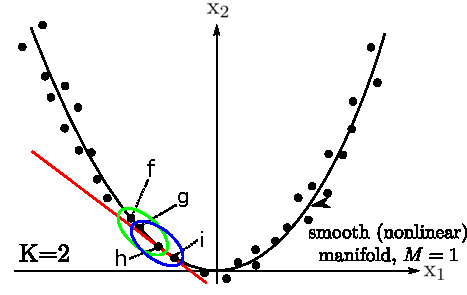
\includegraphics[width=0.2\textwidth]{img/section4_fig11_K2}
     \mode<article>{
	\caption{Basic RNN architecture}
	}
	\label{fig:rnn} 
\end{figure}
\end{frame}
